\documentclass[11pt,letterpaper]{article}

\usepackage[letterpaper,margin=0.70in,includeheadfoot]{geometry}
\usepackage{libertinus}
\usepackage{microtype}
\usepackage{graphicx}
\usepackage{booktabs,tabularx,array}
\usepackage{enumitem}
\usepackage[most]{tcolorbox}
\usepackage{tikz}
\usepackage{xcolor}
\usepackage{fancyhdr,lastpage}
\usepackage{hyperref}
\usepackage{caption}

\newif\ifteacher
\ifdefined\teacheredition
  \teachertrue
\else
  \teacherfalse
\fi

\graphicspath{{../../../Visual-Plan/assets/exports/figures/}{../../../Visual-Plan/assets/diagrams/}}

\definecolor{APBlue}{HTML}{17395C}
\definecolor{APTeal}{HTML}{168C87}
\definecolor{APOrange}{HTML}{C96B32}
\definecolor{APGold}{HTML}{D7A83D}
\definecolor{PaleBlue}{HTML}{EDF4FA}
\definecolor{PaleTeal}{HTML}{EAF6F4}
\definecolor{PaleOrange}{HTML}{FFF1E8}
\definecolor{Ink}{HTML}{1E2F40}
\definecolor{Muted}{HTML}{5E7185}
\definecolor{Answer}{HTML}{3E6B4B}

\hypersetup{colorlinks=true,linkcolor=APBlue,urlcolor=APBlue}
\setlength{\parindent}{0pt}
\setlength{\parskip}{4pt}
\setlist{nosep,leftmargin=1.3em}
\setlist[enumerate]{itemsep=5pt}
\setlength{\tabcolsep}{5pt}
\setlength{\fboxrule}{0.5pt}
\setlength{\fboxsep}{4pt}

\pagestyle{fancy}
\fancyhf{}
\setlength{\headheight}{24pt}
\lhead{\textsf{AP Microeconomics · Unit 1}}
\rhead{\textsf{Session 01 · Scarcity}}
\cfoot{\textsf{\thepage\ / \pageref{LastPage}}}
\renewcommand{\headrulewidth}{0.4pt}
\renewcommand{\headrule}{\hbox to\headwidth{\color{APBlue}\leaders\hrule height \headrulewidth\hfill}}

\newcommand{\blankanswer}[2][0.96\linewidth]{\fcolorbox{APBlue!55}{white}{\makebox[#1][l]{\rule{0pt}{#2}}}}
\newcommand{\answerline}[1][0.96\linewidth]{\par\vspace{2pt}\noindent\blankanswer[#1]{0.32in}\par\vspace{4pt}}
% Table cells need a top-aligned box without the paragraph spacing used by
% standalone response areas.
\newcommand{\tableanswerline}[1][0.96\linewidth]{%
  \begin{minipage}[t]{\linewidth}%
    \vspace{0pt}\noindent
    \smash{\raisebox{0.10in}{\blankanswer[#1]{0.32in}}}%
    \vphantom{\blankanswer[#1]{0.32in}}%
  \end{minipage}%
}
\newcommand{\shortanswer}[1][0.26\linewidth]{\rule{#1}{0.45pt}}
\newcommand{\teachernote}[1]{\ifteacher\begin{tcolorbox}[colback=green!4,colframe=Answer!65!black,title=Teacher note,fonttitle=\bfseries,boxsep=4pt,left=5pt,right=5pt,top=4pt,bottom=4pt]#1\end{tcolorbox}\fi}
\newcommand{\answer}[1]{\ifteacher\textcolor{Answer}{\footnotesize\textbf{Answer:} #1}\fi}
\newcommand{\teacherfill}[1]{\ifteacher\textcolor{Answer}{#1}\else\rule{0.70\linewidth}{0.35pt}\fi}
\newcommand{\studentoranswer}[2]{\ifteacher\textcolor{Answer}{#2}\else #1\fi}

\newtcolorbox{objectivebox}{colback=PaleBlue,colframe=APBlue!80!black,boxrule=0.8pt,arc=2pt,left=7pt,right=7pt,top=6pt,bottom=6pt}
\newtcolorbox{modelbox}{colback=PaleTeal,colframe=APTeal!75!black,boxrule=0.8pt,arc=2pt,left=7pt,right=7pt,top=6pt,bottom=6pt}
\newtcolorbox{warningbox}{colback=PaleOrange,colframe=APOrange!85!black,boxrule=0.8pt,arc=2pt,left=7pt,right=7pt,top=6pt,bottom=6pt}
\newtcolorbox{exitbox}{colback=APBlue!4,colframe=APBlue!75!black,boxrule=0.9pt,arc=2pt,left=7pt,right=7pt,top=6pt,bottom=6pt}

\newcommand{\sectiontitle}[2]{\vspace{2pt}{\color{APBlue}\Large\bfseries #1}\hfill{\color{Muted}\small\textsf{#2}}\par\vspace{3pt}\hrule\vspace{7pt}}
\newcommand{\component}[1]{\textcolor{Muted}{\scriptsize\textsf{#1}}}
\newcommand{\choicebox}[1]{\fbox{\rule{0pt}{1.3em}\hspace{0.4em}#1\hspace{0.4em}}}

\begin{document}

% --------------------------------------------------------------------------
% Page 1
% --------------------------------------------------------------------------
{\color{APBlue}\Huge\bfseries Scarcity and Resource Allocation\par}
\vspace{3pt}
{\color{Muted}\large Unit 1 · Session 01 · 90-minute handout}
\hfill
\textsf{\ifteacher TEACHER KEY\else STUDENT EDITION\fi}

\begin{objectivebox}
\component{H01 · Official targets}\textbf{By the end of this lesson, I can:}
\begin{itemize}
  \item define resources and explain why scarcity creates trade-offs;
  \item answer the allocation questions: what, how, and for whom to produce;
  \item compare how market, command, and mixed systems coordinate scarce resources;
  \item explain one choice with a clearly identified foregone alternative.
\end{itemize}
\textbf{College Board links:} MKT-1.A and MKT-1.B (CED pp. 41--42).
\end{objectivebox}

\sectiontitle{H02 · Retrieval and prediction}{0--8 minutes}
\textbf{1. Classify the resource.} For each item, circle \textbf{scarce}, \textbf{non-scarce in this model}, or \textbf{not enough information}. Give one reason for one of your choices.

\begin{center}
\begin{tabularx}{\linewidth}{@{}>{\raggedright\arraybackslash}p{0.31\linewidth}X@{}}
\toprule
Item & Your classification and reason \\
\midrule
A machine available for one production line at a time & \tableanswerline[0.58\linewidth] \\
Established knowledge that can be used by several producers at once & \tableanswerline[0.58\linewidth] \\
A student's 30-minute lunch break & \tableanswerline[0.58\linewidth] \\
\bottomrule
\end{tabularx}
\end{center}
\answer{Machine: scarce because it has alternative uses and cannot be used by every line at the same time. Established knowledge can be nonrival in this model. Time is scarce because the same minutes cannot be used for two activities simultaneously.}

\textbf{2. Prediction.} A town has a fixed amount of land, labor, and time. If it chooses to produce more school meals, what must happen to at least one other possible use of those resources? Explain in one sentence.
\answerline
\answerline
\answer{At least one alternative use must receive fewer resources or be given up; scarcity creates a trade-off.}

\sectiontitle{Core question}{Why must every society make allocation choices?}
\begin{modelbox}
\textbf{Scarcity} means that available resources are insufficient to satisfy all wants and needs. Scarcity is a condition of limited resources relative to desired uses; it is not the same as poverty, inequality, or a temporary market shortage.

\textbf{A trade-off} is the set of alternatives that must be considered when a scarce resource has more than one possible use. The value of the best alternative given up is the \textbf{opportunity cost}; this phrase is a bridge to the deeper PPC and cost-benefit work in Sessions 2 and 4.
\end{modelbox}

\ifteacher\else\newpage\fi

% --------------------------------------------------------------------------
% Page 2
% --------------------------------------------------------------------------
\sectiontitle{H01 · Core model and vocabulary}{8--30 minutes}

\begin{tabularx}{\linewidth}{@{}>{\bfseries\raggedright\arraybackslash}p{0.22\linewidth}X>{\raggedright\arraybackslash}p{0.25\linewidth}@{}}
\toprule
Term & Student-friendly meaning & Quick check \\
\midrule
Resource & An input used to satisfy wants or produce goods and services. & What is one resource in today's scenario? \\
Scarcity & Resources are limited relative to desired uses. & Does a high price define scarcity? \answer{No.} \\
Trade-off & Choosing one use means giving up another use. & What is the alternative use? \\
Factor of production & Land, labor, capital, or entrepreneurship used to produce output. & Is money itself physical capital? \answer{No.} \\
Physical capital & Produced tools, machines, buildings, and equipment used to produce other goods or services. & Name one example. \\
\bottomrule
\end{tabularx}

\vspace{7pt}
\begin{warningbox}
\textbf{Common traps to avoid}
\begin{itemize}
\item Scarcity exists even when a product is free at the point of use. The scarce input may be land, labor, time, or capacity.
\item Financial capital (money used to finance a purchase) is different from physical capital (a produced input such as a tractor).
\item A shortage is a market outcome at a particular price. Scarcity is the more basic condition that makes choices unavoidable.
\end{itemize}
\end{warningbox}

\ifteacher\newpage\fi
\sectiontitle{H03 · The three allocation questions}{15--30 minutes}
Every economic system must coordinate answers to three questions. Complete the examples for a community clinic with a fixed budget, staff, and building.

\begin{center}
\begin{tabularx}{\linewidth}{@{}>{\bfseries\raggedright\arraybackslash}p{0.22\linewidth}X>{\raggedright\arraybackslash}p{0.27\linewidth}@{}}
\toprule
Question & What the question asks & Clinic example \\
\midrule
What to produce? & Which goods or services will be made? & \shortanswer[0.46\linewidth] \\
How to produce? & Which methods and combinations of inputs will be used? & \shortanswer[0.46\linewidth] \\
For whom to produce? & Who will receive or consume the output? & \shortanswer[0.46\linewidth] \\
\bottomrule
\end{tabularx}
\end{center}
\answer{Examples: what: vaccinations or meal kits; how: nurses and equipment versus a mobile unit; for whom: residents meeting an eligibility rule, patients who pay, or another stated group. Accept any internally consistent answer.}

\textbf{Write the causal chain.} Because the clinic has a fixed amount of \underline{\hspace{1.0in}} and \underline{\hspace{1.0in}}, it cannot provide every possible service at the same time. Therefore, it must decide \underline{\hspace{1.0in}}.

\answer{Possible completion: staff and time; what to produce and for whom to produce.}

\ifteacher\else\newpage\fi

% --------------------------------------------------------------------------
% Page 3
% --------------------------------------------------------------------------
\sectiontitle{P01 · How economic systems coordinate}{30--45 minutes}

\begin{center}
\begin{tabularx}{\linewidth}{@{}>{\bfseries\raggedright\arraybackslash}p{0.19\linewidth}X X X@{}}
\toprule
System & Main coordinating mechanism & Typical ownership / decision pattern & Fill one implication for scarce resources \\
\midrule
Market & Prices, incentives, and voluntary exchange & Private ownership is important; buyers and sellers interact & If demand rises, a higher price can signal producers to reallocate inputs. \\
Command & Central planning and administrative direction & Government or public institutions direct substantial resource use & \shortanswer[0.27\linewidth] \\
Mixed & A combination of markets and government rules or provision & Private and public decisions operate together & \shortanswer[0.27\linewidth] \\
\bottomrule
\end{tabularx}
\end{center}

\textbf{Compare, do not rank.} Complete two sentences.

\begin{enumerate}
\item In a market system, the answer to “what to produce?” is influenced by \shortanswer[0.22\linewidth]
\item In a command system, the answer to “how to produce?” may be influenced by \shortanswer[0.22\linewidth]
\end{enumerate}
\answer{Market: prices, demand, profit incentives, and buyer-seller interaction. Command: a central authority's plan, public ownership, or administrative decisions.}

\begin{modelbox}
\textbf{Worked example.} A city has one vacant lot. It can support a public playground, a parking lot, or a small clinic. A market process might use a price signal and private ownership to coordinate the use. A command process might use a public planning decision. A mixed process might combine public zoning with a private construction decision.

\textbf{Economic reasoning:} The system changes the coordination mechanism; it does not remove scarcity. Every option still uses a limited lot and therefore displaces at least one alternative.
\end{modelbox}

\newpage
\sectiontitle{G02 · Visual model: the resource bundle}{Use the visual, then explain it}
\begin{center}
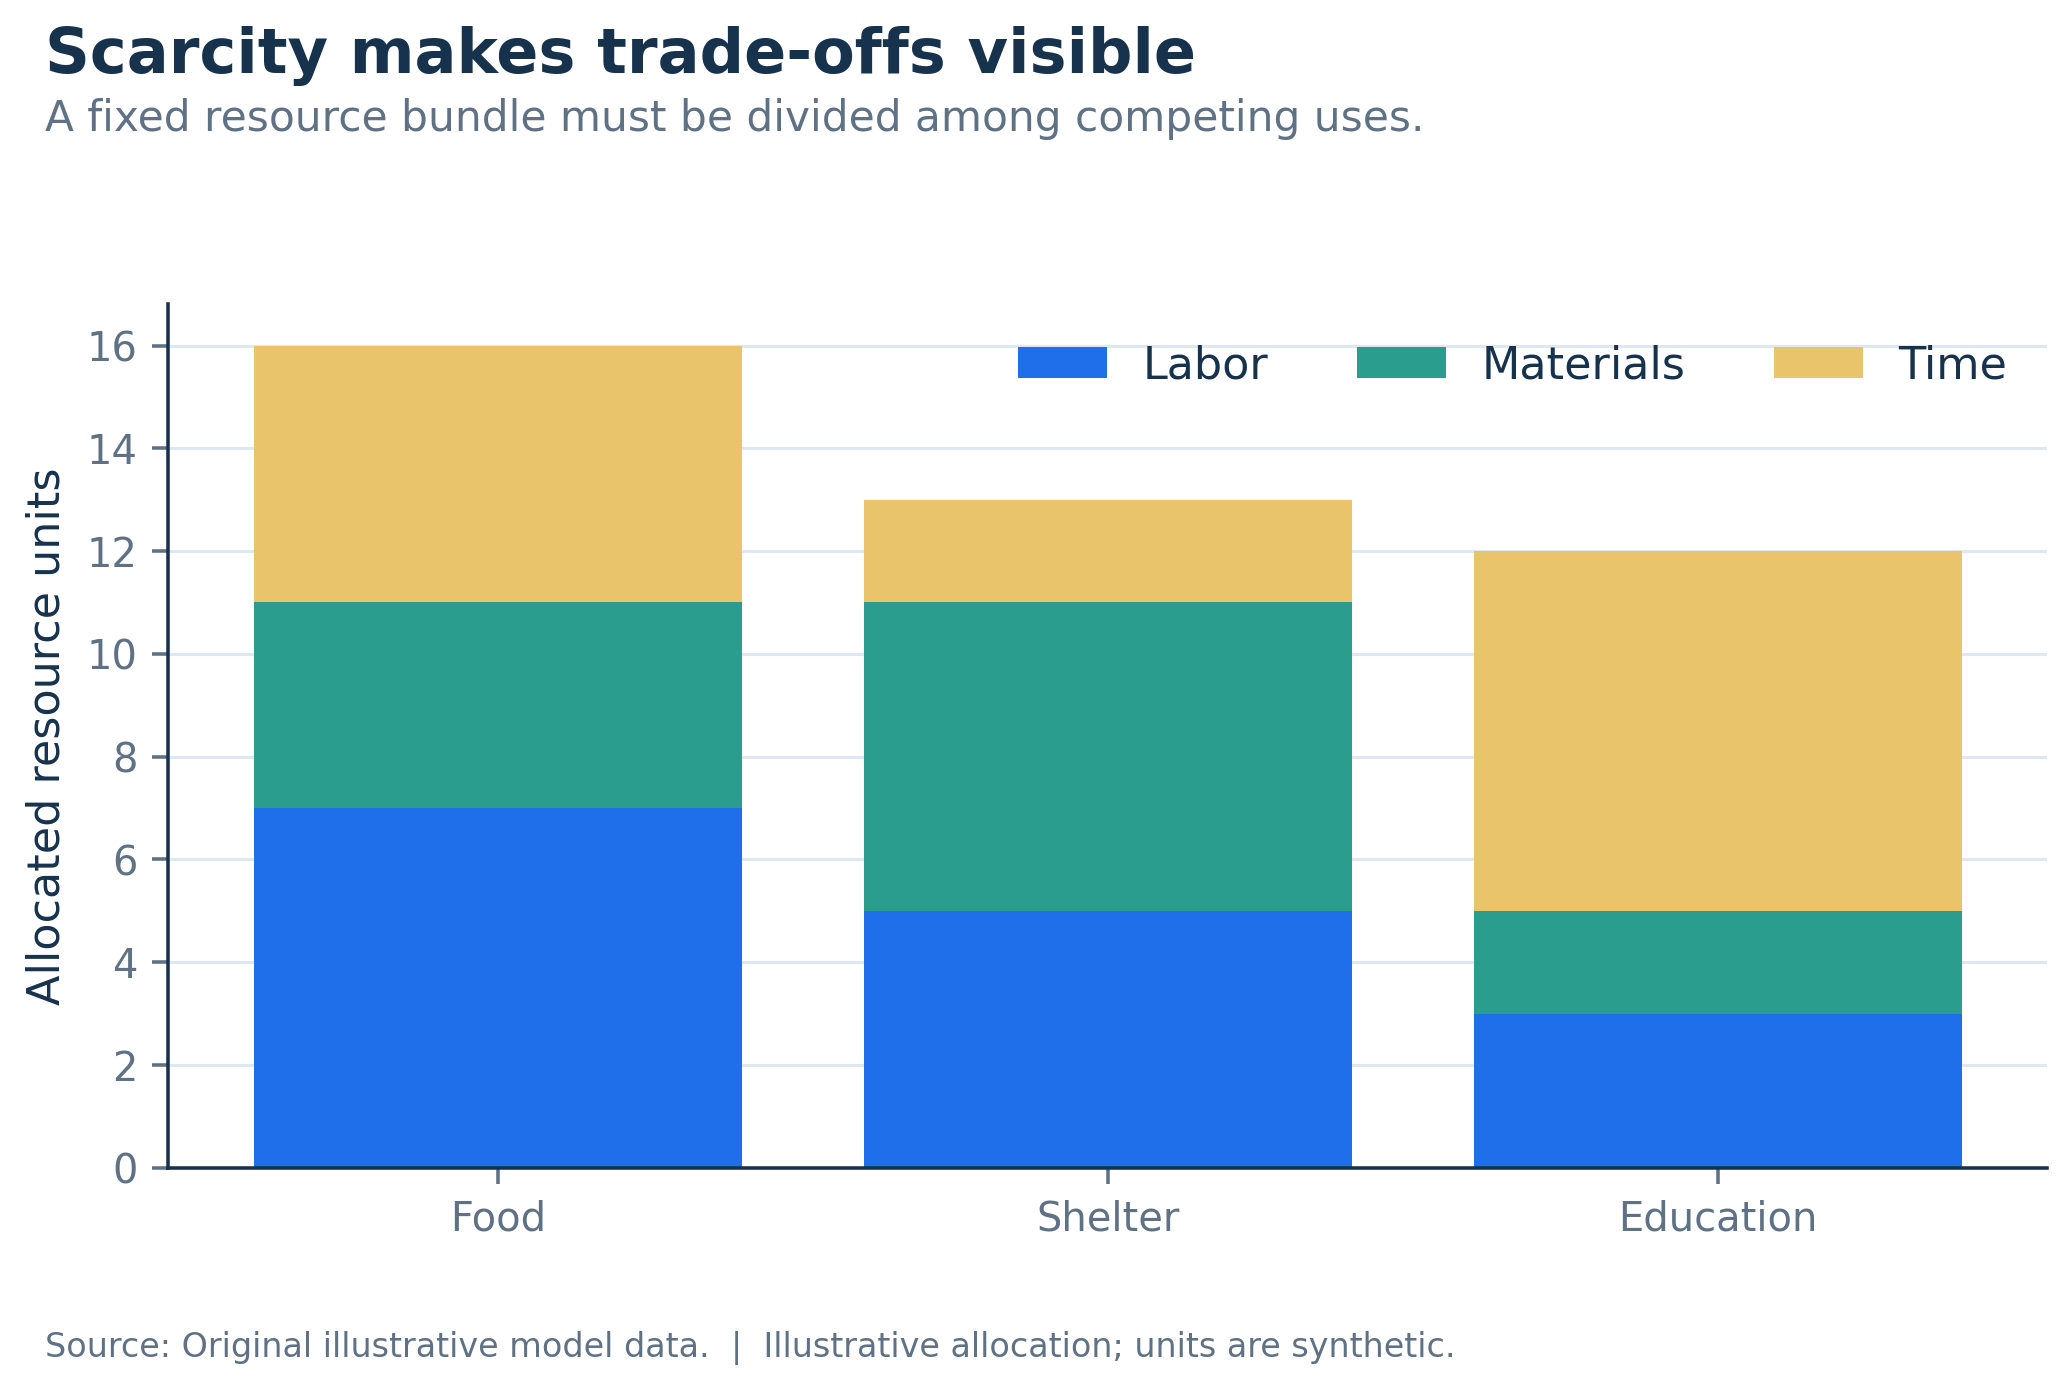
\includegraphics[width=0.72\linewidth]{session-01-three-resource-scarcity-panel.png}
\captionof{figure}{An original illustrative allocation table. The bars show a fixed bundle of labor, materials, and time allocated across competing uses.}
\end{center}

\textbf{Prompt.} Choose one bar. Name one resource in that bar and one alternative use that receives fewer resources when this use expands.

Resource: \shortanswer[0.20\linewidth] \hfill Alternative use: \shortanswer[0.20\linewidth]

\answer{Answers depend on the selected bar. The essential evidence is a fixed resource and a displaced alternative.}

\newpage

% --------------------------------------------------------------------------
% Page 4
% --------------------------------------------------------------------------
\sectiontitle{G01 · Choice and opportunity-cost bridge}{45--60 minutes}
\begin{center}
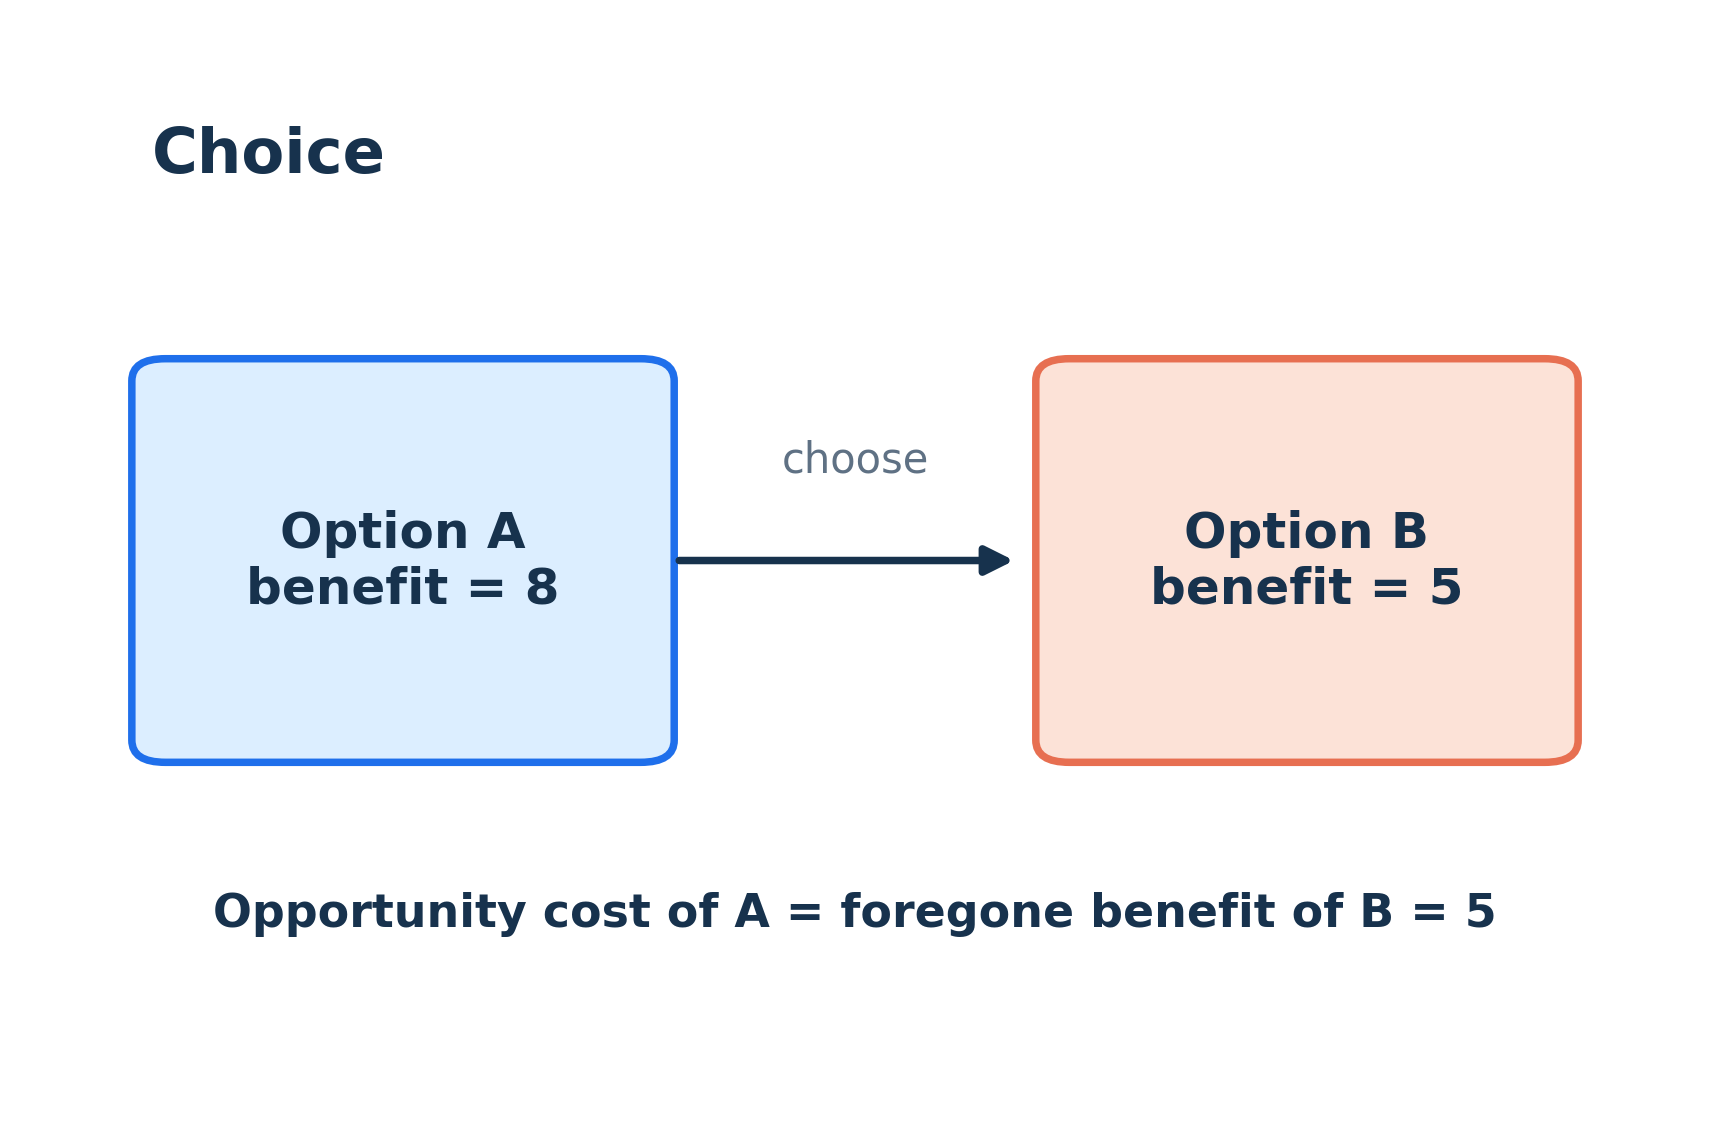
\includegraphics[width=0.70\linewidth]{session-01-choice-opportunity-cost-card.png}
\captionof{figure}{The first choice is visible only when the foregone alternative is named. This bridge supports later PPC and cost-benefit work.}
\end{center}

\textbf{1. Label the choice.} If a decision-maker chooses Option A, the opportunity cost is the benefit of \shortanswer[0.12\linewidth]

\textbf{2. Explain the choice in a complete sentence.} Use the frame:

\begin{modelbox}
Because the decision-maker has a limited \underline{\hspace{1.15in}}, choosing Option A means giving up \underline{\hspace{1.15in}}; therefore, the opportunity cost of A is \underline{\hspace{1.15in}}.
\end{modelbox}
\answer{Because the decision-maker has a limited choice opportunity/resource, choosing A means giving up the benefit from B; therefore, the opportunity cost of A is 5 benefit units.}

\newpage
\sectiontitle{Bridge graph · one trade-off, no new Unit 2 model}{A preview for Session 2}
The diagram below is intentionally a simple production-possibilities sketch. It asks only what a movement along the boundary means. Do not label efficiency, growth, or a changing curve in this lesson.

\begin{center}
\begin{tikzpicture}[x=0.58cm,y=0.40cm]
  \draw[->,thick,APBlue] (0,0) -- (11,0) node[below right] {Good A};
  \draw[->,thick,APBlue] (0,0) -- (0,11) node[above left,align=center] {Good B};
  \draw[very thick,APTeal] (0.5,9.5) .. controls (3.2,8.9) and (6.4,5.8) .. (9.8,0.7);
  \fill[APBlue] (3.2,7.9) circle (2.5pt) node[above right] {A};
  \fill[APOrange] (6.6,4.7) circle (2.5pt) node[above right] {B};
  \draw[densely dashed,Muted] (3.2,0) -- (3.2,7.9) (0,7.9) -- (3.2,7.9);
  \draw[densely dashed,Muted] (6.6,0) -- (6.6,4.7) (0,4.7) -- (6.6,4.7);
\end{tikzpicture}
\end{center}

\textbf{3. As production moves from A to B:}
\begin{enumerate}[label=\alph*)]
\item Which good increases? \shortanswer[0.25\linewidth]
\item Which good decreases? \shortanswer[0.25\linewidth]
\item What is the trade-off? \shortanswer[0.25\linewidth]
\end{enumerate}
\answer{Good A increases, Good B decreases, and the trade-off is the amount of Good B forgone to obtain more Good A. The sketch is qualitative; no numerical opportunity cost is calculated here.}

\begin{warningbox}
\textbf{Boundary reminder.} Session 1 introduces the logic of scarcity and allocation. Session 2 will formalize PPC points, efficiency, underutilization, growth, curvature, and numerical opportunity-cost calculations.
\end{warningbox}

\newpage

% --------------------------------------------------------------------------
% Page 5
% --------------------------------------------------------------------------
\sectiontitle{T01 · AP transfer and E01 · Exit ticket}{60--90 minutes}

\textbf{Transfer 1 — choose the best answer.} A school has one empty classroom and must choose between a tutoring center and a rehearsal room. Which statement is most accurate?

\begin{enumerate}[label=\Alph*.]
\item Scarcity exists only if the school charges rent for the room.
\item The room is scarce because it has alternative uses and cannot serve every use at the same time.
\item There is no scarcity if both activities are valuable to students.
\item A command economy would eliminate the trade-off by making both uses happen simultaneously.
\end{enumerate}
Answer: \choicebox{A}\choicebox{B}\choicebox{C}\choicebox{D}

Evidence from the prompt: \shortanswer[0.22\linewidth]
\answer{B. The fixed classroom has alternative uses. Its value does not depend on whether a fee is charged, and a different coordinating system cannot create a second room.}

\textbf{Transfer 2 — short response.} A city council sets a rule that a public building will become a clinic. Identify which allocation question is being answered and explain how the decision illustrates scarcity.

Allocation question: \shortanswer[0.22\linewidth]

Because → therefore → result: \answerline[0.96\linewidth]
\answer{“What to produce?” The building and its staff/time have alternative uses, so choosing a clinic means some other service is forgone.}

\textbf{Transfer 3 — system comparison.} A government owns most factories and sets production targets. Which coordinating mechanism is most directly described? Explain one contrast with a market system.

Mechanism: \shortanswer[0.22\linewidth]
Contrast: \shortanswer[0.22\linewidth]
\answerline[0.96\linewidth]
\answer{Command coordination; a central authority directs resource use. In a market system, prices, incentives, and buyer-seller interaction play a larger role.}

\ifteacher\newpage\fi
\sectiontitle{E01 · Exit ticket}{last 3 minutes}
\begin{exitbox}
\textbf{Complete both lines.}

The key relationship from today is: \answerline[0.96\linewidth]

If \underline{\hspace{1.2in}} changes, then \underline{\hspace{1.2in}} because \underline{\hspace{1.2in}}.

One point I still need to check: \answerline[0.96\linewidth]
\end{exitbox}
\answer{Accept any accurate causal sentence linking a scarce resource to a choice, trade-off, or allocation mechanism.}

\teachernote{Collect this page. Sort responses into concept, graph, reading, calculation, or expression errors. For this first lesson, most useful evidence is whether students name the displaced alternative and distinguish the three allocation questions from the economic system used to coordinate them.}

\end{document}
